\chapter{Tipologías Estructurales}
\section{Introducción.}
El término tipo estructural hace referencia al ``conjunto de elementos resistentes capaz de mantener sus formas y cualidades a lo largo del tiempo, bajo la acción de las cargas y agentes exteriores a que ha de estar sometido''. (Torroja)

Es importante conocer las formas resistentes de los diferentes tipos estructurales para poder determinar el tipo estructural ``óptimo'' que se ajuste a todas las exigencias de la construcción: función utilitaria, función estructural, exigencias estéticas y limitaciones económicas.

El proyectista debe elegir el tipo estructural que, dentro de las condiciones que le impone la finalidad de la construcción a la que pertenece, resulta más adecuado y económico para construirlos con los materiales y técnicas disponibles.

En el tipo estructural influyen diferentes aspectos: el material empleado, los procesos constructivos, la geometría. Fijado el material y el proceso constructivo, la escala fija la relación entre las acciones actuantes, las resistencias y las rigideces necesarias.

No hay solución única: una misma geometría y una misma carga con diferentes rigideces y resistencias produce diferentes distribución de esfuerzos y desplazamientos.

En relación con la escala:
\begin{itemize}
    \item El peso de la estructura crece con el volumen ($\lambda_L^3$)
    \item La resistencia y la rigidez dependen del área de la sección transversal ($\lambda_L^2$)
    \item Cuando variamos la escala de una estructura, su peso crece con el cubo de sus dimensiones, pero la sección transversal que debe soportar ese peso aumenta sólo con el cuadrado de las dimensiones. 
    \item Cuando el peso propio es muy importante no se puede incrementar la forma proporcionalmente: se pierde la semejanza geométrica a menos que se usen mejores materiales.
\end{itemize}

\begin{figure}[h]
    \centering
    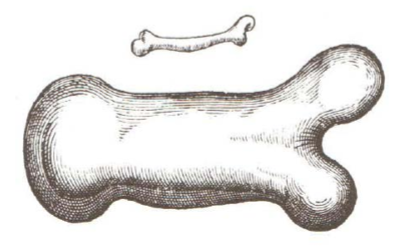
\includegraphics[width=0.75\linewidth]{Imagenes/Galileo Galilei.png}
    \caption{Hueso de perro y de caballo (Dibujo de Galileo Galilei, 1638).}
\end{figure}

En relación con la geometría:
\begin{itemize}
    \item Aunque la geometría es sólo un aspecto de la tipología estructural, a veces es fundamental para ``filtrar'' esfuerzos. Ejemplos: el cable sólo soporta tracciones.
    \item Hay dos características importantes de la geometría que determinan los mecanismos resistentes movilizados para soportar las cargar: la curvatura y el alabeo.
    \begin{itemize}
        \item Curvatura: toda superficie cortada por planos que pasan por la recta perpendicular a ella en un punto muestra dos direcciones perpendiculares entre sí (direcciones principales de curvatura para las cuales la curvatura resulta máxima y mínima, respectivamente. La envolvente de las direcciones principales de curvatura en cada punto forman las líneas principales de curvatura. Las superficies con una curvatura principal nula y la otra del mismo signo en todos los puntos se llaman desarrollables (se pueden aplanar sin cortarlas).
        \item Alabeo: diferencia de pendientes entre lados opuestos de su geometría. Cualquier elemento rectangular de superficie cuyos lados sean paralelos a las direcciones principales de curvatura no tiene alabeo.
    \end{itemize}
\end{itemize}

En relación con elementos estructurales y estructura en su conjunto, a la hora de abordar su proyecto y cálculo han de considerarse tres aspectos:
\begin{itemize}
    \item Equilibrio: ha de asegurarse la inmovilidad de la estructura en conjunto, y de cada una de sus partes por separado, respecto al cimiento que lo sustenta.
    \item Resistencia: El material ha de ser capaz, en todos y cada uno de sus volúmenes elementales de la estructura, de soportar las fuerzas internas a que se le somete como resultado del estado de carga general y de las acciones locales de cada fuerza exterior.
    \item Estabilidad: Hay que evitar fenómenos de pandeo o inestabilidad global.
\end{itemize}

En relación con la resistencia:
\begin{itemize}
    \item Las fuerzas exteriores se transmiten y equilibran a través del sólido estructural creando en cada punto o elemento diferencial del mismo un estado tensional.
    \item Sobre cada plano que pasa por ese punto actúa una tensión que varía en general en intensidad y en inclinación al variar la orientación del plano.
    \item Siempre hay tres orientaciones perpendiculares entre sí (direcciones principales) sobre las cuales las tensiones que actúan son normales al plano (tensiones principales).
    \item De los valores de esas tensiones principales depende que el cuerpo pueda resistir o no el estado tensional.
    \item Las envolventes de las direcciones principales forman la red de líneas isostáticas que permiten una buena representación del estado tensional.
    \item Puede imaginarse que a través de las líneas isostáticas el sólido se acorta o alarga en proporción a la tensión (de tracción o de compresión) actuante*.
    \item No confundir direcciones principales de curvatura (en superficies) con direcciones principales de tensiones; las primeras dependen sólo de la geometría mientras que las segundas depende también de las cargas aplicadas y de las condiciones contorno. 
\end{itemize}

\section{Elementos estructurales y esfuerzos básicos actuantes.}
\subsection{Clasificaciones.}
\subsubsection{Clasificación según su geometría.}
\begin{itemize}
    \item Sin curvatura (elementos lineales y losas)
    \begin{itemize}
        \item Monodimensionales
        \begin{itemize}
            \item Cables: elementos de tracción.
            \item Barras comprimidas biarticuladas: elementos a compresión.
        \end{itemize}
        \item Bidimensionales
        \begin{itemize}
            \item Losas: se caracterizan porque las cargas actuales y condiciones de contorno generan en un punto del plano medio de la losa dos grupos de esfuerzos
            \begin{itemize}
                \item Grupo 1: Esfuerzos contenidos en plano medio: $N_X , N_Y, N_{XY}$
                \item Grupo 2: Esfuerzos perpendiculares plano medio: $M_X, M_Y, M_{XY}, M_{YX}, V_X, V_Y$.
            \end{itemize}
            Casos particulares de losas según los esfuerzos que generen las acciones y condiciones contorno:
            \begin{itemize}
                \item Laja: sólo esfuerzos del Grupo 1.
                \item Placa: sólo esfuerzos del Grupo 2.
            \end{itemize}
            \item Superficies / láminas plegadas: formadas por planos unidos por sus bordes.
        \end{itemize}
    \end{itemize}
    \item Con curvatura (láminas)
    \begin{itemize}
        \item Láminas de simple curvatura (en una de las direcciones principales de curvatura, la curvatura es nula)
        \begin{itemize}
            \item Arcos (monodimensionales)
            \item Bóvedas (bidimensionales)
        \end{itemize}
        \item Láminas de doble curvatura:
        \begin{itemize}
            \item Del mismo signo (sinclásticas)
            \item De diferente signo (anticlásticas)
        \end{itemize}
    \end{itemize}
    Una lámina general se caracteriza porque las acciones exteriores y las condiciones de contorno generan esfuerzos en el plano tangente a cada punto, del Grupo 1 ($N_X , N_Y, N_{XY}$) y del Grupo 2 ($M_X, M_Y, M_{XY}, M_{YX}, V_X, V_Y$). Casos particulares de láminas:
    \begin{itemize}
        \item Membrana: sólo esfuerzos del Grupo 1: $N_X , N_Y, N_{XY}$
        \item Lámina a flexión pura: solo esfuerzos del Grupo 2: $M_X, M_Y, M_{XY}, M_{YX}, V_X, V_Y$
    \end{itemize}
\end{itemize}

\subsubsection{Clasificación según la dirección de transmisión de la carga.}
\begin{itemize}
    \item Transferencia unidireccional de la carga:
    \begin{itemize}
        \item De directriz recta: cable, barra a tracción / compresión, viga.
        \item De directriz no recta: arco, arco funicular.
    \end{itemize}
    \item Transferencia bidireccional de la carga
    \begin{itemize}
        \item Sin curvatura: entramados, lajas, placas o losas, estructuras espaciales.
        \item Con curvatura: láminas, bóvedas, cúpulas, paraboloides.
    \end{itemize}
\end{itemize}

\subsection{Elementos unidimensionales (transferencia unidireccional de la carga).}
\subsubsection{Elementos sometidos a tracción y compresión.}
\paragraph{Cables.}
Son elementos de pequeña dimensión transversales en relación con su longitud. Trabajan sometidos a esfuerzos de tracción. Ventaja: uso completo de la sección; eficiencia y economía. Inconveniente: su adaptabilidad a las cargas cambiantes los hace inestables. En los puentes colgantes las armaduras que cuelgan del cable, además de sostener la calzada deben conferir rigidez a los cables frente a movimientos debidos a cargas cambiantes o móviles.

\begin{itemize}
    \item Cable sometido a una carga vertical: para soportarla debe formar ángulo con la horizontal. La flecha óptima (mínimo volumen de cable para una distancia horizontal $D$ dada) es $D/2$.
    \item Cable sometido a varias cargas verticales: éste adopta una configuración de equilibrio con lados rectos entre las cargas y cambios de dirección en los puntos de aplicación de éstas que se llama polígono funicular (es la forma natural de soportar cargas por tracción).
    \item Cable sometido a un número elevado de cargas verticales: su forma de equilibrio se aproxima a una curva continua llamada curva funicular.
    \begin{itemize}
        \item Si todas las cargas son iguales y están separadas horizontalmente la misma distancia la curva funicular es una parábola. La flecha óptima para un cable parabólico es $D/3$.
        \item Si todas las cargas son iguales y se distribuyen a distancias iguales a lo largo del cable la curva funicular es una catenaria. La flecha óptima para una catenaria es aprox. $D/3$.
    \end{itemize}
    Para la flecha óptima, la parábola y la catenaria son muy parecidas.
\end{itemize}

\begin{figure}[h]
    \centering
    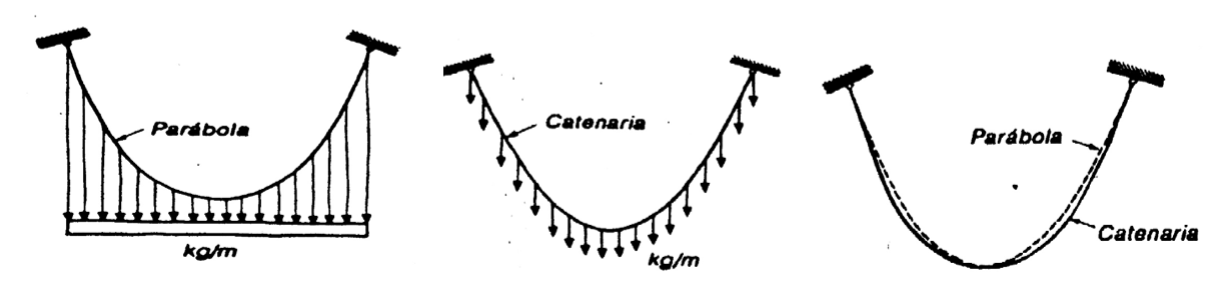
\includegraphics[width=\linewidth]{Imagenes/Catenaria y parabola.png}
\end{figure}

\paragraph{Barras a compresión y arcos funiculares.}
Si se invierte la estructura de tracción pura formada por un cable y una carga vertical, y se dimensionan las barras para que trabajen a compresión, se obtiene una estructura formada por barras trabajando bajo esfuerzos de compresión pura. Las barras (esbeltas) sometidas a compresión pueden pandear, generándose esfuerzos de flexión inducidos: al ir aumentando la carga de compresión se alcanza un valor (carga de pandeo) para el cual la barra además de acortarse se curva (pandea). La carga de pandeo de una barra depende del material, de su longitud, de la sección transversal y de las restricciones impuestas en los extremos. Si se invierte el polígono o la curva parabólica que toma el cable baja cargas iguales distribuidas uniformemente en dirección horizontal se obtiene una forma ideal de arco llamado arco funicular que sometido a ese tipo de carga desarrolla sólo esfuerzos de compresión.

\begin{figure}[h]
    \centering
    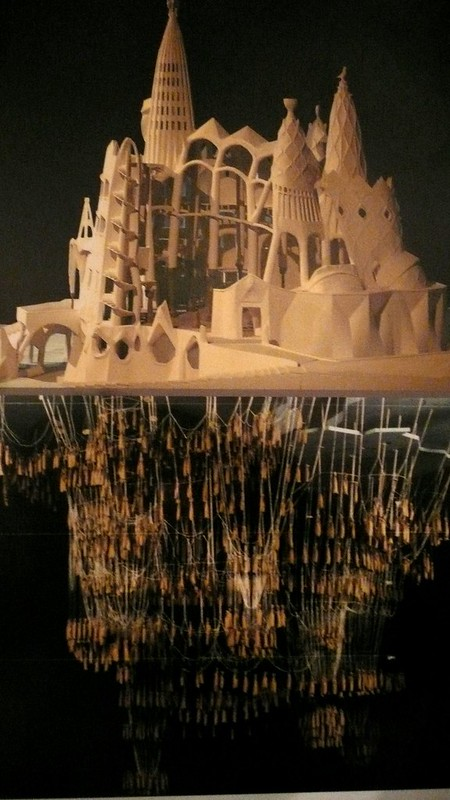
\includegraphics[width=0.75\linewidth]{Imagenes/Gaudi.png}
    \caption{Arcos funiculares. Catedral de la Sagrada Familia, Barcelona.}
\end{figure}

\subsubsection{Elementos sometidos a flexión.}
\paragraph{Vigas}
Son uno de los elementos estructurales de uso más común. Su mecanismo resistente implica una combinación de esfuerzos de flexión y de cortante (acción de viga). Si la viga tiene impedidos los desplazamientos de los extremos en la dirección longitudinal, se desarrollan también esfuerzos de tracción (acción de cable)

\subparagraph{Viga en Voladizo (sección rectangular).}
Flexión: tensiones normales y deformación.
\begin{figure}[H]
    \centering
    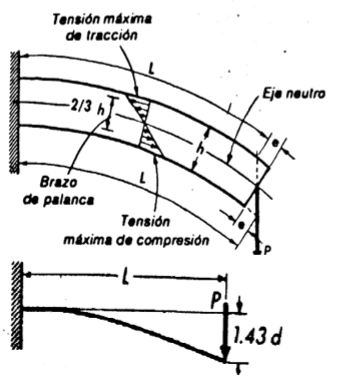
\includegraphics[width=0.75\linewidth]{Imagenes/Viga en voladizo seccion rectangular - flexion.png}
\end{figure}

Cortante: tensiones tangenciales y deformación.
\begin{figure}[H]
    \centering
    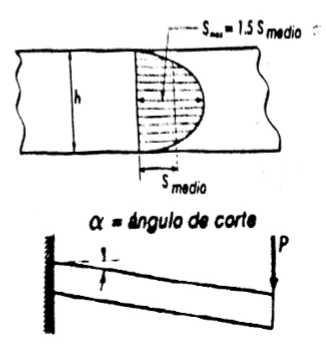
\includegraphics[width=0.75\linewidth]{Imagenes/Viga en voladizo seccion rectangular - Cortante.png}
\end{figure}

\subparagraph{Viga en Voladizo (perfil I).}
La sección rectangular es poco eficiente a flexión ya que la mayoría de las fibras no trabajan a la tensión máxima (sólo las extremas). Se puede aumentar la eficiencia disponiendo la mayor parte del material en extremos: perfil I. En los perfiles I las alas resisten fundamentalmente la flexión y el alma el cortante. Si el alma y/o el ala comprimida del perfil I son demasiado delgadas pueden pandear. El ala comprimida pandea curvándose en su propio plano horizontal (el alma le impide hacerlo en plano vertical) y la sección experimenta una rotación: pandeo lateral flexión/torsión. Las tensiones tangenciales que genera el cortante, y estas compresiones pueden provocar el pandeo local del alma.
\begin{figure}[H]
    \centering
    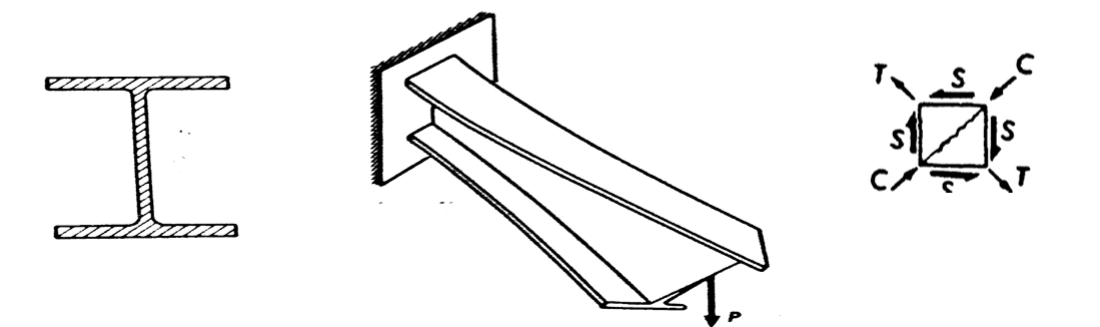
\includegraphics[width=\linewidth]{Imagenes/Viga en voladizo perfil I.png}
\end{figure}

\subparagraph{Viga Biapoyada.}
Isostáticas (régimen elástico).
\begin{figure}[H]
    \centering
    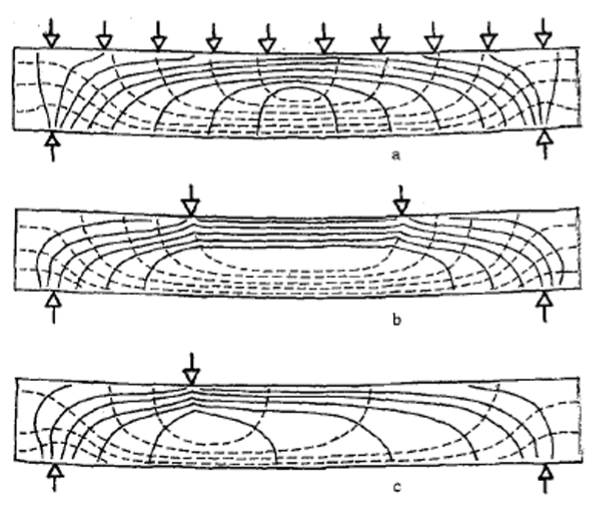
\includegraphics[width=0.75\linewidth]{Imagenes/Viga Biapoyada - Isostaticas.png}
\end{figure}

Reserva de resistencia por redistribución de tensiones(régimen plástico).
\begin{figure}[H]
    \centering
    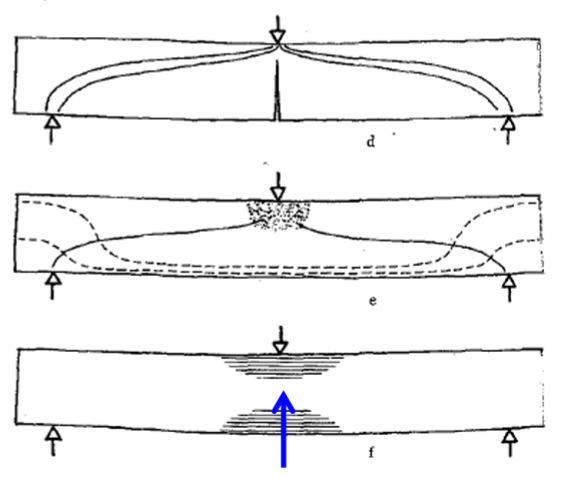
\includegraphics[width=0.75\linewidth]{Imagenes/Viga Biapoyada - resistencia.png}
\end{figure}

\subparagraph{Viga Biapoyada con extremos inmovilizados.}
Con un extremo libre (sólo acción de viga).
\begin{figure}[H]
    \centering
    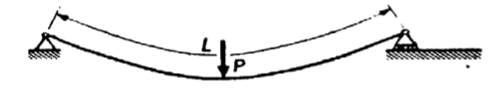
\includegraphics[width=0.75\linewidth]{Imagenes/Viga biapoyada con un extremo inmobilizado.png}
\end{figure}
Con ambos extremos inmovilizados (acción de viga + acción de cable).
\begin{figure}[H]
    \centering
    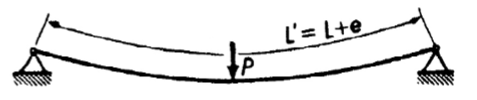
\includegraphics[width=0.75\linewidth]{Imagenes/Viga biapoyada con ambos extremos inmovilizados.png}
\end{figure}
La flexión de la viga requiere un alargamiento $e$ de la fibra medida que genere tracciones en ella.
Cuando se forma un número suficiente de rótulas plásticas y la viga se convierte en un mecanismo, es incapaz de soportar mayores cargas por acción viga, pero puede seguir haciéndolo por acción cable.

\subsection{Elementos bidireccionales (transferencia bidireccional de la carga).}
\subsubsection{Entramados rectangulares (emparrillados).}
Consisten en una retícula de vigas dispuestas en dos direcciones. Se movilizan esfuerzos de flexión, cortante y torsión. 

\paragraph{Transmisión de una carga entre dos vigas perpendiculares con unión no rígida.}
Dos vigas perpendiculares apoyadas en sus extremos y unidas entre sí no rígidamente pero de forma que en su intersección sufran igual deformación, transmiten la carga a los apoyos repartiéndosela según su rigidez a flexión. En el caso de vigas de distinta longitud, para obtener una transmisión eficiente en dos direcciones, la viga más larga debe tener mayor inercia.

\paragraph{Transmisión de varias cargas entre vigas perpendiculares con unión no rígida.}
Los puntos de intersección de las vigas sufren igual desplazamiento vertical.

\paragraph{Transmisión de varias cargas entre vigas perpendiculares con unión rígida.}
Si las conexiones entre vigas con uniones rígidas se introduce una nueva acción estructural en el entramado: la deformación de flexión en las secciones de una viga genera torsiones (alabeo) en las secciones de la viga perpendicular. Esta nueva acción estructural aumenta la rigidez del conjunto, reduciéndose los desplazamientos del entramado. Con entramados se puede llegar de forma económica a relaciones espesor/luz de 1/30 o 1/40, mientras que en sistemas convencionales con transmisión unidireccional de la carga oscila entre 1/1o y 1/24. En la práctica el entramado se completa con una loseta superior lo que le da monolitismo y aumenta las ventajas de la acción bidireccional. El mecanismo de torsión que se genera puede transmitir parte de la carga.

\subsubsection{Losas.}
Es un elemento superficial monolítico de espesor relativamente pequeño. Su forma de trabajo se puede asimilar a la de un entramado de infinitas vigas rígidamente unidas y que trabajan en cualquier dirección (idealmente la losa puede dividirse en franjas que conecten dos puntos cualquiera del perímetro de apoyo), buscando el mecanismo más eficiente de transmisión de las cargas (el de menores tensiones). 
\begin{itemize}
    \item Acción de plaza: puede entenderse como equivalente a una acción de viga  (movilizando esfuerzos flectores y cortantes) en dos direcciones, sumada a la acción de torsión (esfuerzos torsores) distribuida uniformemente en la placa.
    \item La acción de torsión transfiere un \% importante (el 50\% en placas cuadradas) de la carga aplicada.
\end{itemize}

\paragraph{Reserva de resistencia en losas.}
Los elementos estructurales bidimensionales como las losas tienen una reserva de resistencia proveniente de dos fuentes separadas: redistribución de tensiones y acción de membrana.
\begin{itemize}
    \item Redistribución de tensiones. A medida que aumenta la carga, las secciones más solicitadas redistribuyen las tensiones en su espesor (fluencia plástica), provocando aumentos de tensiones en las secciones próximas y la fluencia de líneas enteras de secciones (líneas de articulación). La losa puede desarrollar múltiples líneas de articulación hasta alcanzar la carga máxima (formación de mecanismo).
    \item Acción de membrana. En casi todos los casos, las superficies que adoptan las losas al deformar son superficies no desarrollables, y eso hace que el plano medio de la losa tenga que estirarse para adquirir esas deformaciones, desarrollándose esfuerzos de tracción (acción membrana) capaces de resistir cierta carga. La acción membrana se produce incluso cuando los lados de la losa pueden moverse libremente, pero es mucho mayor cuando están impedidos. Es el equivalente bidimensional de la acción cable (unidimensional).
\end{itemize}

\paragraph{Losa cuadrada simplemente apoyada en los lados con carga uniforme.}
La red de isostáticas (direcciones principales) dan el ``recorrido'' de las tensiones normales debidas a la flexión.

\paragraph{Losas nervadas.}
La eficiencia de la losa se puede aumentar disponiendo la mayor cantidad de material a cierta distancia del plano medio (neutro), creando nervaturas en una, dos (forjados reticulares) o más direcciones (p.e. siguiendo las isostáticas).

\begin{figure}[h]
    \centering
    \includegraphics[width=\linewidth]{Imagenes/Losas nervadas.png}
    \caption{The Palazzo del Lavoro, Turin, 1959-1961.}
\end{figure}

\subsubsection{Láminas plegadas.}
La eficiencia de la placa se puede aumentar disponiendo la mayor cantidad de material a cierta distancia del ``plano medio''.

\begin{figure}[h]
    \centering
    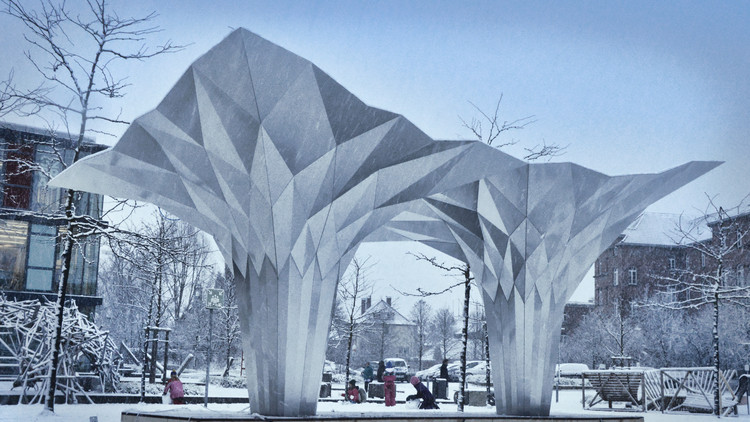
\includegraphics[width=1\linewidth]{Imagenes/Laminas plegadas.png}
    \caption{Origami pavilion by Tal Friedman Architecture.}
\end{figure}

\paragraph{Placa plegada consistente en placas en ángulo sobre pórticos/muros extremos.}
Dos placas en ángulo se pueden asimilar a una viga rectangular equivalente. La acción de placa plegada es una combinación de viga transversal y viga longitudinal.

\paragraph{Acción de placa plegada.}
Una franja ideal de placa se comporta como una viga transversal contina apoyada en los pliegues, en los cuales aparecen reacciones verticales R, que a su vez pueden dividirse en componentes en los planos propios de las placas. Las reacciones R se transmiten a los pórticos/muros extremos a través de los pares de placas en ángulo que trabajan como grandes vigas longitudinales (asimilables a vigas rectangulares equivalentes).

\subsubsection{Membranas.}
Elementos bidimensionales con curvatura y de muy poco espesor sometidos a acciones exteriores y con condiciones de contorno bajo las cuales desarrollan sólo esfuerzos contenidos en el plano tangente de cada punto ($N_X, N_Y, N_{XY}$). Soporta las cargas (acción de membrana) a través de dos mecanismos resistentes que pueden desarrollarse por el carácter bidimensional del elemento y por su geometría (curvaturas y alabeo):

\begin{itemize}
    \item Mecanismo o acción de cable en dos direcciones ortogonales (que son las propias direcciones principales de tensiones), debido a las curvaturas (diferencia de pendientes entre puntos de un mismo lado) de su geometría. La acción cable en la dirección principal de mayor ratio $r = flecha/luz$ (mayor curvatura) absorbe más carga que la dirección de menor $r$ (menor curvatura).
    \item Mecanismo o acción de corte dentro de la superficie de la membrana, debida al alabeo (diferencia de pendientes entre lados opuestos) de su geometría.
\end{itemize}

\subsubsection{Láminas (cáscaras delgadas).}
Elementos bidimensionales con curvatura y de muy poco espesor, sometidos a acciones exteriores y con condiciones de contorno que generan esfuerzos en el plano tangente a cada punto tanto en su plano $(N_X, N_Y, N_{XY})$ como perpendiculares al plano $M_X, M_Y, M_{XY}, M_{YX}, V_X, V_Y$.

Deben su eficiencia a la curvatura y al alabeo, que movilizan distintos mecanismos (acción membrana = acción cable + acción de corte).

Clasificación según criterios geométricos:
\begin{itemize}
    \item Superficies de revolución: rotación de una curva plana alrededor de eje vertical cortando (cono, esfera, elíptica, parabólica, etc.) o no al eje (toro).
    \item Superficies de traslación: traslación de una curva plana sobre otra curva plana (cilindro, paraboloide elíptico, paraboloide hiperbólico...)
    \item Superficies regladas: desplazamiento de un segmento de recta sobre dos curvas separadas (cilindro, cono, paraboloide hiperbólico, superficie conoidal, hiperboloide de una hoja)
    \item Superficies complejas: se obtienen combinando las superficies anteriores (cilindros cruzados,...)
\end{itemize}

\begin{figure}[h]
    \centering
    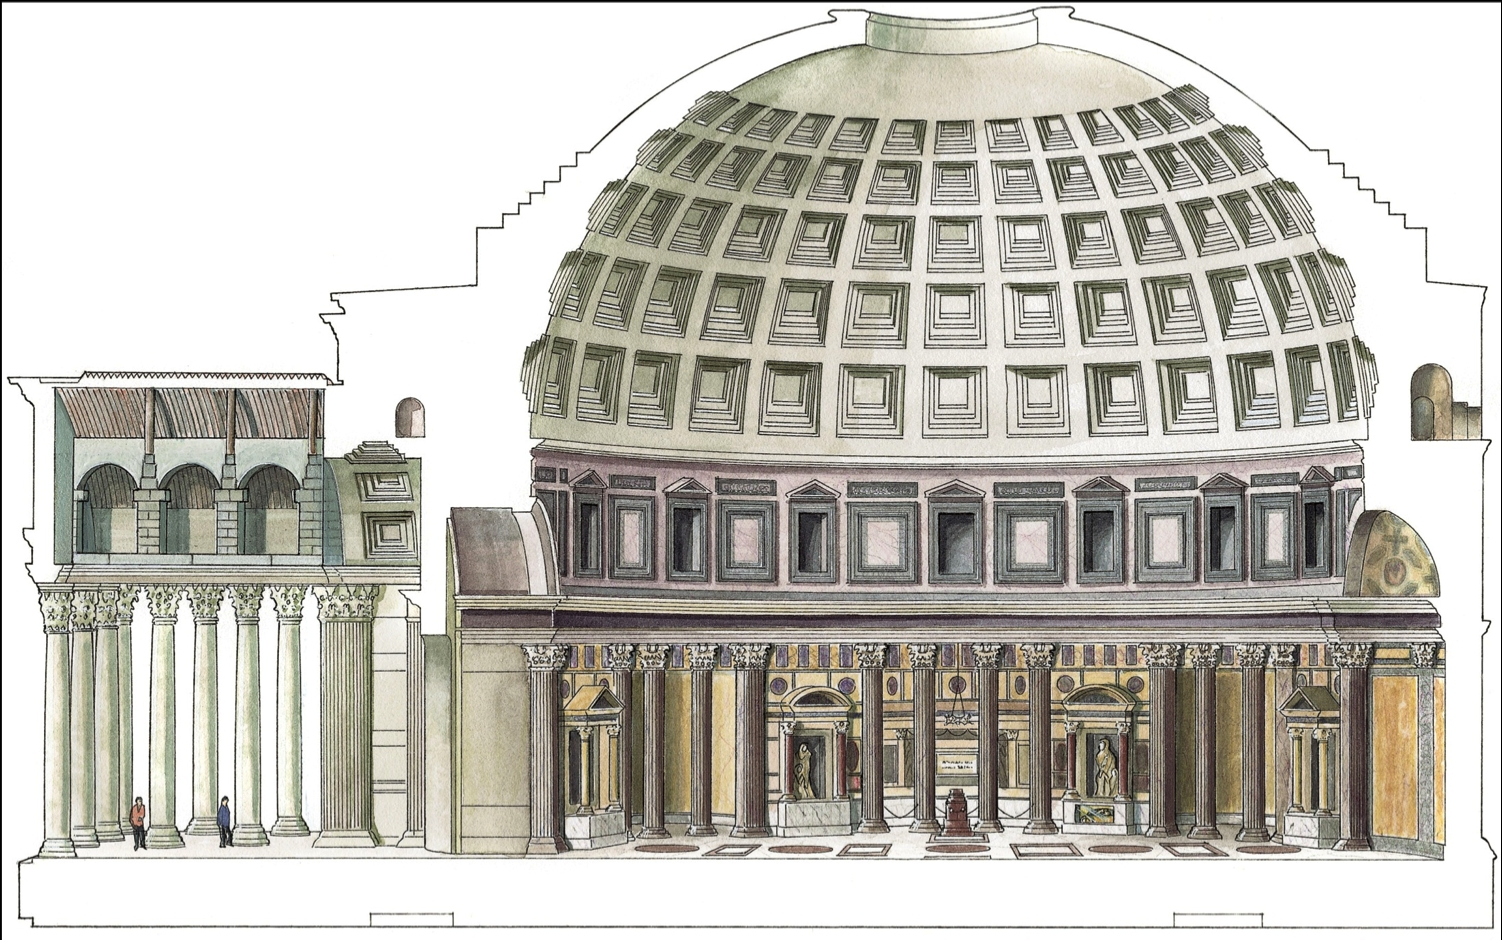
\includegraphics[width=1\linewidth]{Imagenes/Panteon.png}
    \caption{Cúpula del Panteón de Roma - Giovanni Paolo Panini, 1747.}
\end{figure}

\begin{figure}[h]
    \centering
    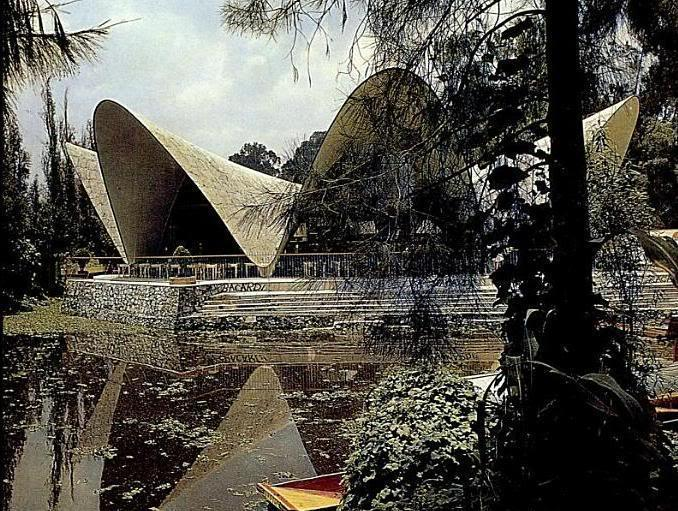
\includegraphics[width=1\linewidth]{Imagenes/Jardines de Xochimilco.png}
    \caption{Restaurante ``Los Manantiales''. Jardines de Xochimilco (1958).}
\end{figure}

\section{Estructuras y sus fundamentos resistentes.}
Nos vamos a ocupar ahora de estructuras en su conjunto, que se obtienen combinando elementos estructurales (de igual o distinta tipología). En general, las estructuras pueden estar formadas por:
\begin{itemize}
    \item Elementos lineales (barras) donde predomina una dimensión: ej. pórticos.
    \item Elementos superficiales: ej. estructuras abovedadas
    \item Macizos de tres dimensiones comparables (semejantes): ej. Presas
\end{itemize}
Nos centramos en los dos primeros tipos.

\subsection{Soluciones convencionales para estructuras de edificación.}
\subsubsection{Sistemas para acciones verticales.}
\paragraph{Pórticos + forjados unidireccionales.}
Combinan elementos lineales (vigas, pilares y viguetas) que transmiten la carga unidireccionalmente. Las vigas y pilares se enlazan mediante uniones rígidas formando pórticos. Las viguetas se enlazan monolíticamente mediante una losa superior de hormigón de poco espesor armada con un mallado formando forjados unidireccionales. El forjado unidireccional puede sustituirse por una ``placa unidireccional''.

\begin{figure}[H]
    \centering
    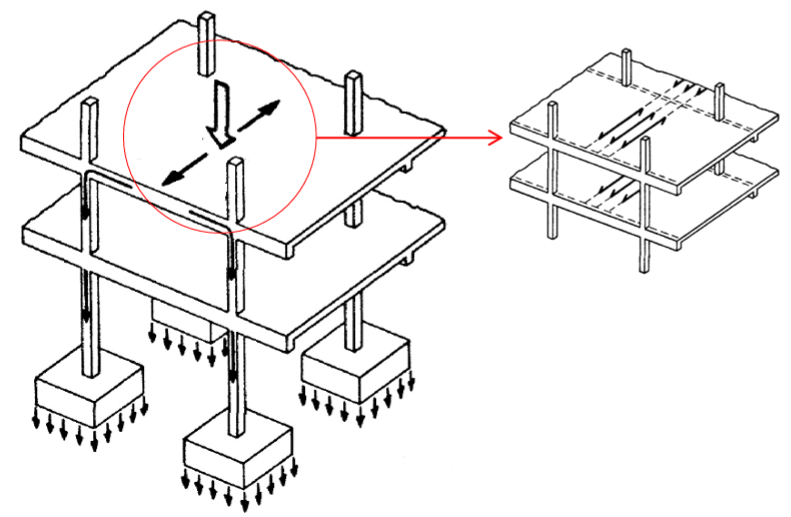
\includegraphics[width=0.75\linewidth]{Imagenes/Porticos+forjados unidireccionales.png}
\end{figure}

\paragraph{Pórticos + placas.}
Combinan elementos lineales (vigas, pilares) conectados mediante uniones rígidas formando pórticos, y elementos bidimensionales (placas) que transmiten la carga bidireccionalmente. Son adecuados para grandes luces y en especial para edificios industriales.

\begin{figure}[H]
    \centering
    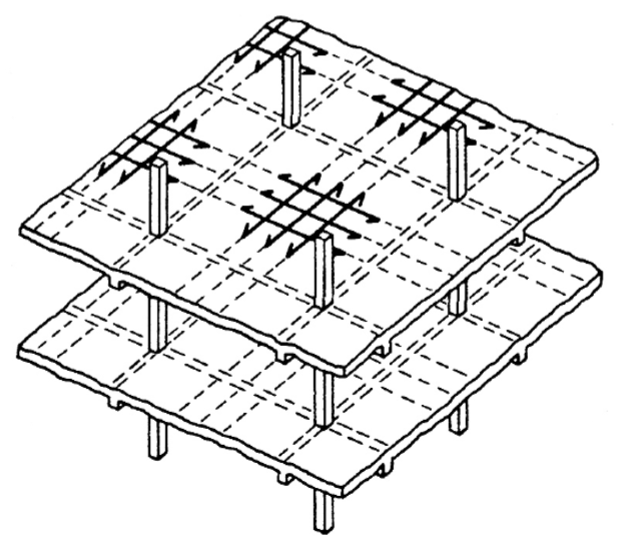
\includegraphics[width=0.75\linewidth]{Imagenes/Porticos + placas.png}
\end{figure}

\paragraph{Placas sobre pilares aislados.}
Combinan elementos lineales (pilares) y elementos bidimensionales (placas) macizos o aligerados, que transmiten la carga bidireccionalmente. La unión entre ambos es una unión rígida. Adecuados para grandes luces y dan libertad para organizar los pilares en planta.

\begin{figure}[H]
    \centering
    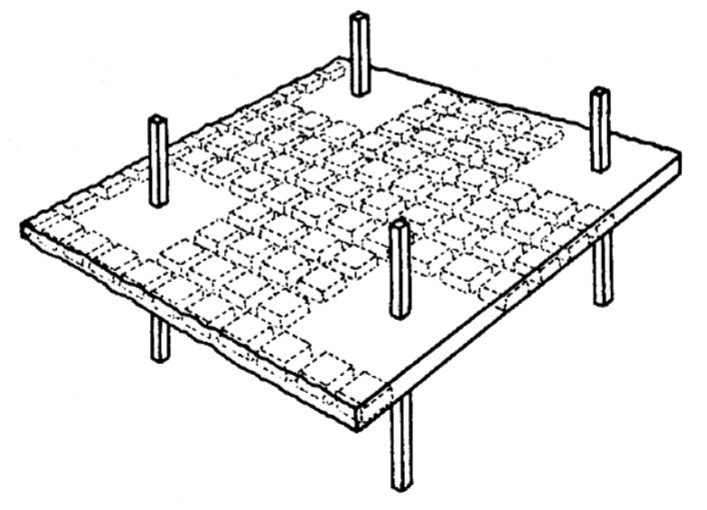
\includegraphics[width=0.75\linewidth]{Imagenes/Placas sobre pilares aislados.png}
\end{figure}

\subsubsection{Sistemas para acciones horizontales.}
\paragraph{Pórticos + forjados/placas.}
Esta solución empleada normalmente para cargas verticales es también eficiente para cargas horizontales cuando éstas no son excesivas o la altura del edificio no es muy elevada. Los forjados funcionan como grandes vigas horizontales, repartiendo las acciones horizontales entre los pórticos, lo cual se conoce como acción diafragma. Los desplazamientos horizontales de la estructura son la suma de dos tipos de deformación global del pórtico: deformación por flexión + deformación por cortante.

\begin{figure}[H]
    \centering
    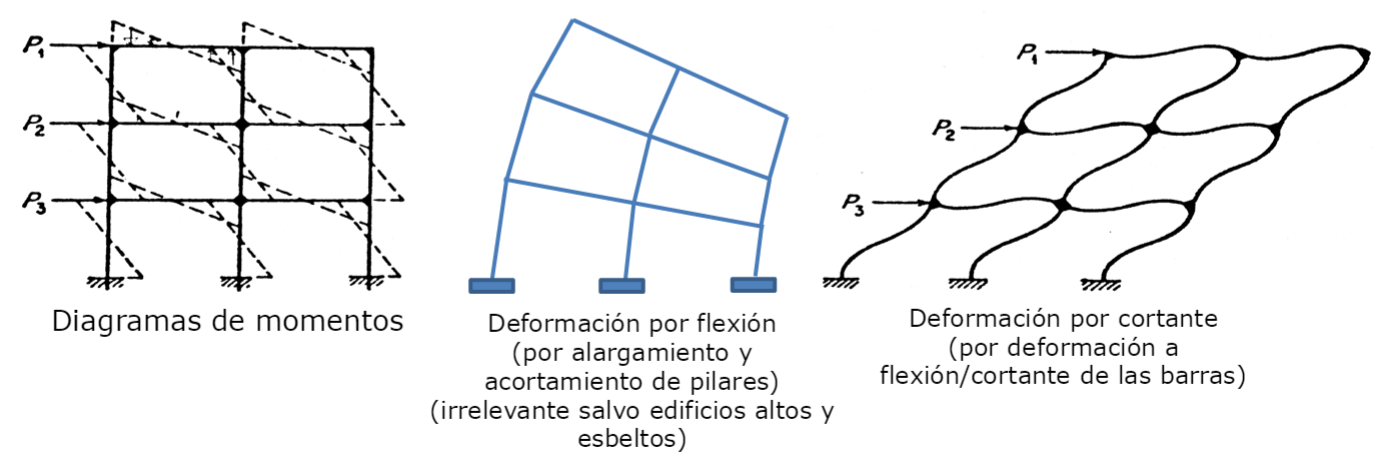
\includegraphics[width=1\linewidth]{Imagenes/Porticos + forjados.png}
\end{figure}

\paragraph{Pantallas + forjados/placas.}
Combinan elementos bidimensionales (pantallas) que trabajan como grandes vigas verticales en voladizo, con forjados o placas que funcionan como grandes vigas horizontales. Los forjados o placas reparten las acciones horizontales entre las pantallas mediante la acción diafragma. Es eficiente para cargas horizontales importante o edificios en altura. Los desplazamientos horizontales de la estructura son debidos fundamentalmente (salvo en pantallas muy poco esbeltas) a la deformación por flexión de la pantalla.

\begin{figure}[H]
    \centering
    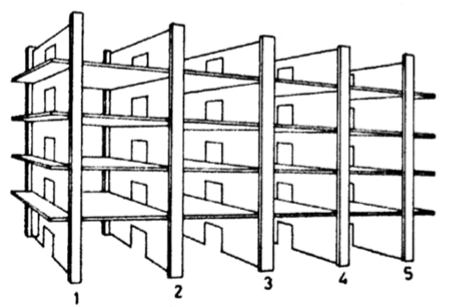
\includegraphics[width=0.75\linewidth]{Imagenes/Pantallas + forjados.png}
\end{figure}

\paragraph{Pórticos + pantallas/núcleos con forjados/placas.}
Se hace trabajar en ``paralelo'' (sometidos a los mismos desplazamientos horizontales) elementos bidimensionales (pantallas) con pórticos conectados con uniones rígidas. Los forjados/placas reparten las acciones horizontales mediante la acción diafragma. Se produce un efecto de interacción pórtico-pantalla.

\begin{figure}[H]
    \centering
    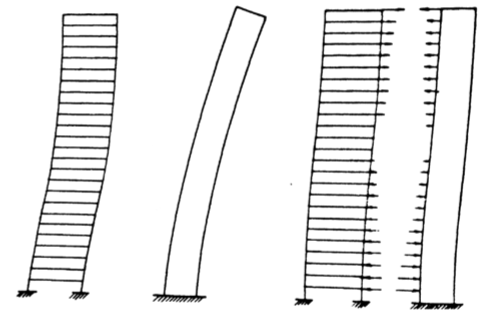
\includegraphics[width=0.75\linewidth]{Imagenes/Porticos + nucleos con forjados.png}
\end{figure}

\paragraph{Pórticos + triangulaciones + forjados/placas.}
Combinan elementos unidimensionales (pilares, vigas y barras inclinadas), formando pórticos (vigas y pilares), con triangulaciones (barras inclinadas) que confieren rigidez y resistencia lat. Los forjados/placas reparten las acciones horizontales mediante la acción diafragma. El ``camino'' para conducir las fuerzas horizontales desde el vuelo del edificio hasta la cimentación es doble: (i) a través de solicitaciones de flexión en las barras del pórtico, y (ii) mediante solicitaciones axiales en las barras inclinadas. Según predominen el primer (i) o el segundo (ii) camino, la estructura resultante será más o menos dúctil, respectivamente. Es importante cómo se distribuyen las triangulaciones en el alzado del pórtico especialmente cuando se trata de edificios muy altos. Disponer los arriostramientos en el mismo vano en todas las plantas puede generar reacciones excesivas en la cimentación

\noindent \underline{Pórticos con triangulaciones en el mismo vano.}
\begin{figure}[H]
    \centering
    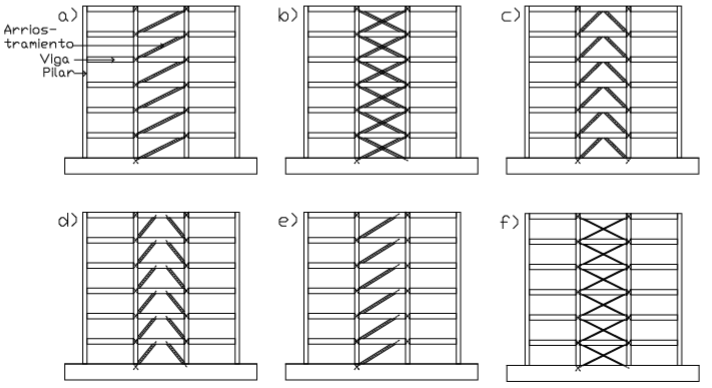
\includegraphics[width=1\linewidth]{Imagenes/Porticos con triangulaciones en el mismo vano.png}
\end{figure}

\noindent \underline{Pórticos con triangulaciones en distintos vanos.}

La solución (a) reduce las reacciones excesivas en la cimentación. Las soluciones (b) y (c) reducen las deformaciones globales por flexión del edificio. En la solución (b) se forman grandes vigas horizontales cada determinado número de plantas que incrementan la colaboración de las columnas más exteriores a resistir el momento de vuelco actuuante en la estructura.

\begin{figure}[H]
    \centering
    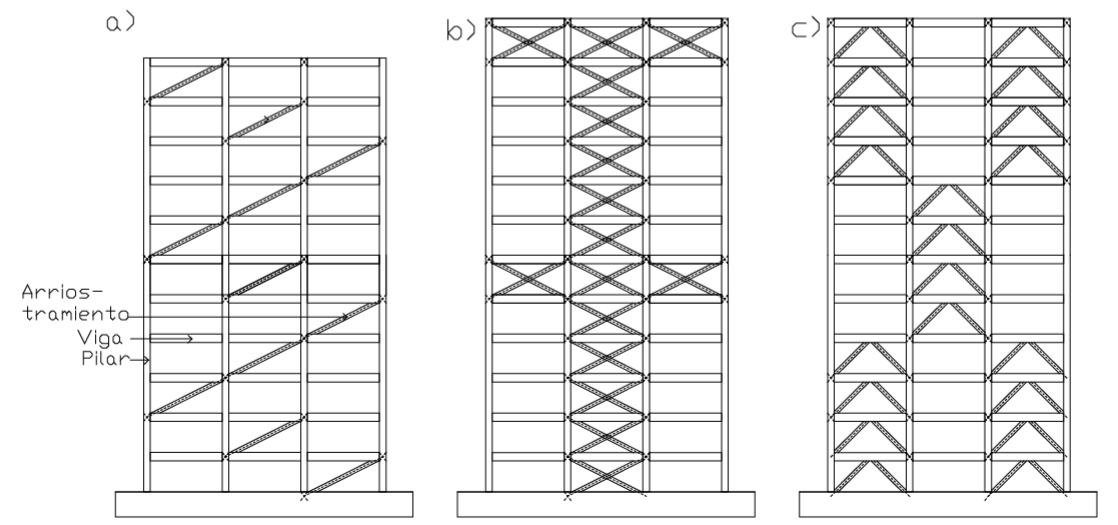
\includegraphics[width=1\linewidth]{Imagenes/Porticos con triangulaciones en distintos vanos.png}
\end{figure}

\noindent \underline{Pórticos excéntricos.}

Consisten en pórticos arriostrados con barras diagonales dispuestas de forma que, en uno o ambos extremos, su eje no concurre al centro del nudo viga-pilar sino a un punto intermedio de la viga, dejando un segmento corto de viga de longitud $e$ sometido a fuertes solicitaciones cortantes (shear links). Se emplean como solución frente a terremotos. Se busca por ello:
\begin{itemize}
    \item Plastificar de zonas muy  concretas de las vigas (en los shear links) y concentrar en ellas los daños estructurales.
    \item Reducir la rigidez lateral.
\end{itemize}

\begin{figure}[H]
    \centering
    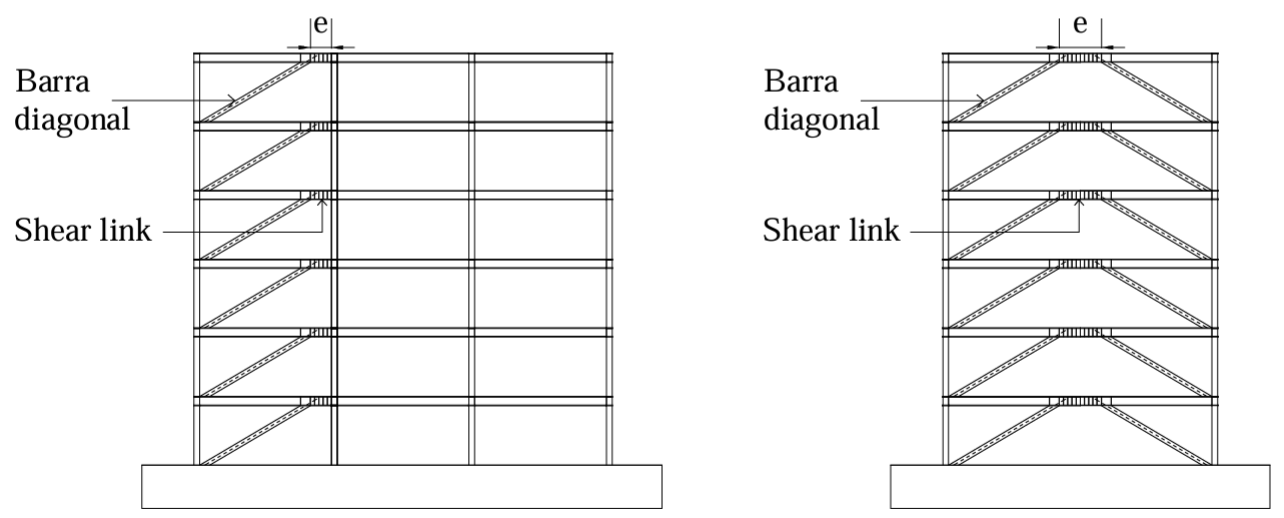
\includegraphics[width=1\linewidth]{Imagenes/Porticos excentricos.png}
\end{figure}

\paragraph{Pantallas acopladas + forjados/placas.}
Se hace trabajar en ``paralelo'' varias conectadas rígidamente con vigas (de acoplamiento). Los forjados/placas reparten las acciones horizontales mediante la acción diafragma. Se emplea como solución frente a terremotos. Las vigas de acoplamiento son proyectadas y armadas para que tengan una elevada capacidad de deformación en régimen plástica. Se busca concentrar las demandas de disipación de energía en un número limitado de partes de la estructura (en vigas de acoplamiento y en arranque de muros).

\begin{figure}[H]
    \centering
    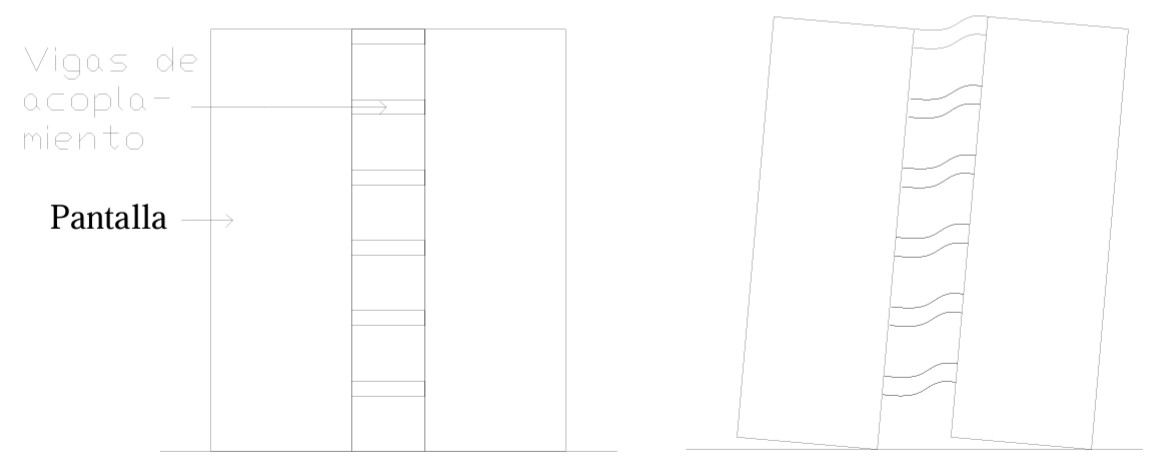
\includegraphics[width=1\linewidth]{Imagenes/Pantallas acopladas + forjados.png}
\end{figure}

\paragraph{Núcleos, tubos y ``tubo en tubo''.}
Los núcleos o tubos se forman uniendo varias pantallas por los lados y se emplean en edificios altos y esbeltos.
\begin{itemize}
    \item Núcleos: se suelen combinar con pórticos (a) y su funcionamiento estructural es similar al visto para pantallas + pórticos.
    \item Tubos: pueden abrirse huecos y constituir la propia fachada del edificio (framed tube structures), convirtiéndose en una retícula densa de ``pilares'' separados 1-3cm y ``vigas'' de 0.25-0.75m de luz y 1-1.5m de canto. 
\end{itemize}

\begin{figure}[H]
    \centering
    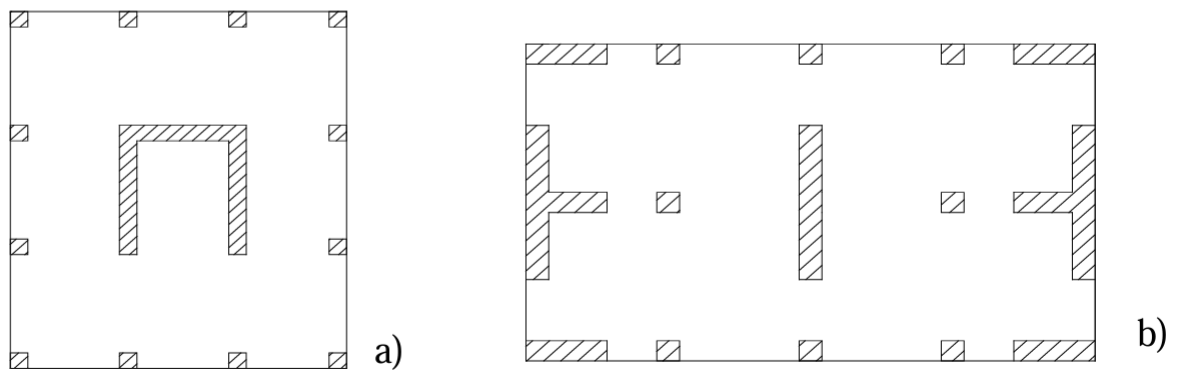
\includegraphics[width=1\linewidth]{Imagenes/Nucleos tubos y tubo en tubo.png}
\end{figure}

\noindent \underline{Tubos: funcionamiento estructural. ``Shear lag effect''.}
El funcionamiento estructural del tubo es similar al de los perfiles tubulares de pared delgada y se caracteriza porque se produce una fuerte concentración de esfuerzos en las ``esquinas'' del tubo por efecto de las deformaciones debidas al esfuerzo cortante (shear lag effect).

\paragraph{Deformaciones de forjados/placas en estructuras bajo acciones horizontales.}
Cuando la unión entre forjados/placas y el resto de la estructura es monolítica y los forjados/placas son suficientemente rígidos en su plano, éstos pueden considerarse a efectos de cálculo como un sólido rígido que se traslada y gira sin deformarse en su propio plano, pero sí perpendicularmente a él (acción diafragma rígido). EHE-08: espesor$\geq$50mm, mallazo, $(L/h)\leq4$. Si el diafragma no es rígido el reparto de las acciones horizontales entre los planos estructurales verticales debe hacerse considerando el forjado/placa como una viga horizontal sobre apoyos elásticos en dichos planos estructurales.

\paragraph{Efectos $P-\Delta$.}
Son las solicitaciones adicionales que aparecen en los elementos estructurales producidos por las acciones gravitatorias con los desplazamientos horizontales de la estructura debidos a las cargas laterales. La carga vertical $P_{tot}$ actuando en la posición deformada induce un momento adicional:
\begin{equation}
    M_{ext} = P_{tot} \Delta
\end{equation}
Una fracción $V_i'$ de la fuerza recuperadora lateral total que opone la estructura debe emplearse en resistir el momento adicional $M_{ext}$, es decir:
\begin{equation}
    P_{tot} \Delta = V_i' h
\end{equation}
operando:
\begin{equation}
    k' = V_i'/ \Delta = P_{tot} / h
\end{equation}
$k'$ representa una rigidez lateral y se puede interpretar como la ``reserva'' de rigidez lateral que debe tener la estructura para compensar el efecto $P-\Delta$.

\begin{figure}[H]
    \centering
    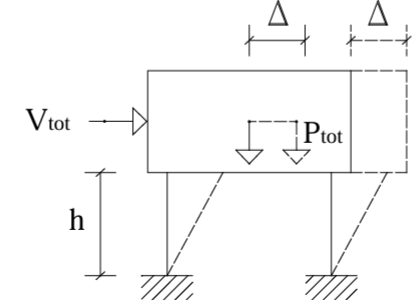
\includegraphics[width=0.5\linewidth]{Imagenes/Efecto P Delta.png}
\end{figure}

\subsection{Soluciones convencionales para obras civiles.}
\subsubsection{Puentes. Tablero, sistema primario y subestructuras.}
Desde el punto de vista morfológico, estructural y constructivo un puente convencional puede descomponerse en tres partes:
\begin{itemize}
    \item Tablero: recibe directamente las sobrecargas de uso debidas al tráfico.
    \item Sistema primario: soporta el tablero y transmite las cargas a los apoyos (vigas, arcos...)
    \item Subestructuras: incluyen pilas y estribos con sus correspondientes cimentaciones; aseguran la transición de las cargas desde el sistema primario hasta el terreno.
\end{itemize}
Al tablero + sistema primario se le denomina también superestructura.

\begin{figure}[H]
    \centering
    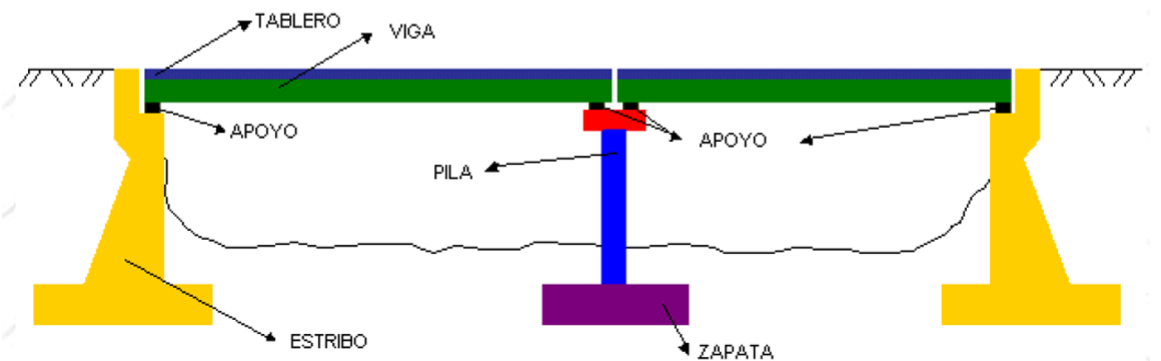
\includegraphics[width=1\linewidth]{Imagenes/Puentes.png}
\end{figure}

\paragraph{Puente arco.}
El sistema primario es un arco apoyado en los extremos de la luz. Las cargas se transmiten mediante compresión del arco hasta los apoyos donde se transforman en una carga horizontal y una vertical. Según el tablero se apoye o cuelgue del arco se tienen tres tipos de puentes arco:
\begin{itemize}
    \item Puente arco con tablero inferior (Fig. \ref{fig:Puente arco con tablero inferior}). 
    \item Puente arco con tablero intermedio (Fig. \ref{fig:Puente arco con tablero intermedio}).
    \item Puente arco con tablero superior (Fig. \ref{fig:Puente arco con tablero superior}).
\end{itemize}

\begin{figure}[h]
    \centering
    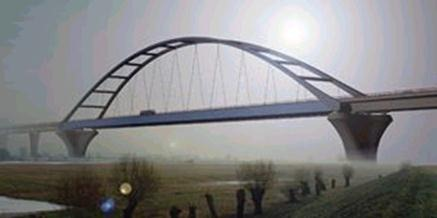
\includegraphics[width=1\linewidth]{Imagenes/Puente de Tangermunde.png}
    \caption{Puente de Tangermunde sobre el Elba (Alemania), F.Leonhardt.}
    \label{fig:Puente arco con tablero inferior}
\end{figure}

\begin{figure}[h]
    \centering
    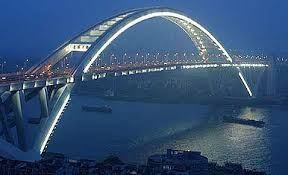
\includegraphics[width=1\linewidth]{Imagenes/Puente Lupu.png}
    \caption{Puente Lupu en Shangay.}
    \label{fig:Puente arco con tablero intermedio}
\end{figure}

\begin{figure}[h]
    \centering
    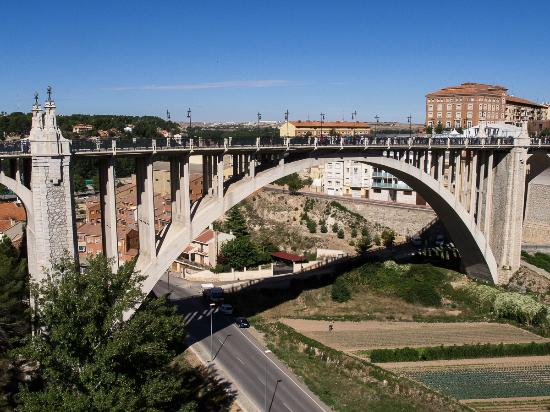
\includegraphics[width=1\linewidth]{Imagenes/Viaducto de hormigon de teruel.png}
    \caption{Viaducto de hormigón de Teruel.}
    \label{fig:Puente arco con tablero superior}
\end{figure}

\paragraph{Tablero sobre soportes o muros.}
El sistema primario es una viga continua (de sección en l, cajón...) o losa continua. La subestructura son pilas y estribos. El apoyo del sistema primario sobre las pilas/estribos es normalmente mediante dispositivos que permiten el desplazamiento horizontal (elastómeros...) para resolver problemas de dilataciones y sísmicos.

\paragraph{Puentes colgantes (Fig. \ref{fig:Puente colgante}).}
El sistema primario es un cable principal apoyado en torres, del que se suspende el tablero mediante tirantes verticales. El tablero suele resolverse con una estructura de acero reticulada y tiene entre sus funciones la de estabilizar los cables.

\begin{figure}[h]
    \centering
    \includegraphics[width=1\linewidth]{Imagenes/Golden gate bridge .png}
    \caption{Golden Gate Bridge.}
    \label{fig:Puente colgante}
\end{figure}

\paragraph{Puentes atirantados (Fig. \ref{fig:Puente atirantado}).}
El sistema primario está formado por tirantes (cables) y torres. Los tirantes introducen importantes fuerzas horizontales en el tablero que deben se absorbidas por éste. Admite numerosas variables:
\begin{itemize}
    \item Asimétricos con una torre, o simétricos con dos torres.
    \item Uno o dos planos de atirantamiento.
    \item Tirantes dispuestos en ``arpa'' o en ``abanico''.
    \item Muchos tirantes poco espaciados o pocos tirantes muy espaciados.
    \item Torres que se inician en los cimientos; o torres que se inician en el tablero formando un conjunto tablero-torres-tirantes apoyados sobre pilas convencionales.
    \item Torres de diferentes formas: una o dos pilas, en forma de A y H o Y invertida...
\end{itemize}

\begin{figure}[h]
    \centering
    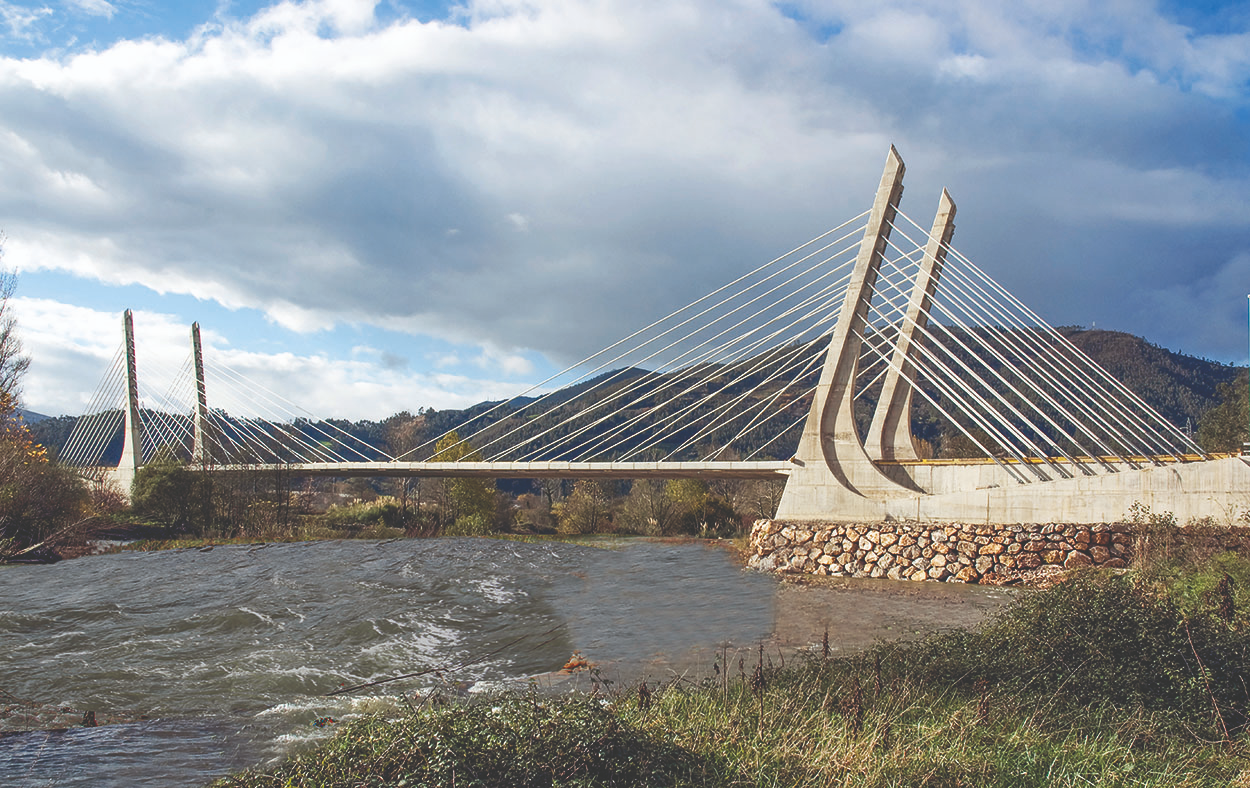
\includegraphics[width=1\linewidth]{Imagenes/Puente sobre el rio Besaya.png}
    \caption{Puente sobre el río Besaya, Cantabria - España.}
    \label{fig:Puente atirantado}
\end{figure}

\paragraph{Puentes en voladizo (Fig. \ref{fig:Puente en voladizo}).}
La estructura principal la forman grandes voladizos pueden servir de apoyo a tramos suspendidos.

\begin{figure}
    \centering
    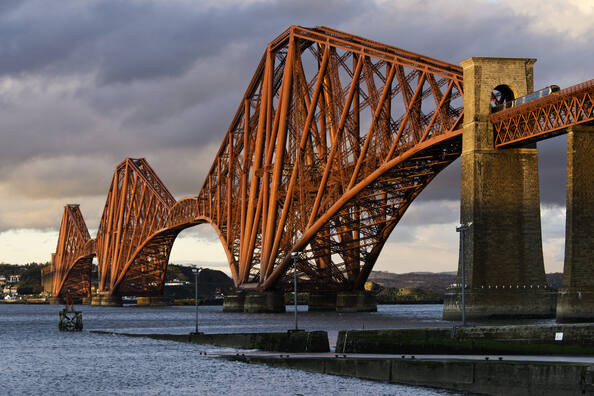
\includegraphics[width=1\linewidth]{Imagenes/Puente Forth.png}
    \caption{Puente Forth, Escocia.}
    \label{fig:Puente en voladizo}
\end{figure}

\subsubsection{Túneles.}
La geometría de la sección transversal consta de 3 superficies: línea de excavación total, línea de sostenimiento (o casa exterior) y línea de revestimiento (o cara interior). Partes estructurales de un túnel: bóveda hastiales o muros laterales y contrabóveda o solera. Los túneles se pueden excavar por dos procedimientos:
\begin{itemize}
    \item Mediante voladura de explosivos: la energía potencial liberada en la detonación se transforma en energía cinética y mecánica.
    \item Excavación mecánica: se aplica fuerza provocando la indentación y rotura terreno; puede hacerse con máquinas de ataque (rozadoras; excavadoras) o con tuneladoras.
\end{itemize}

\begin{figure}[H]
    \centering
    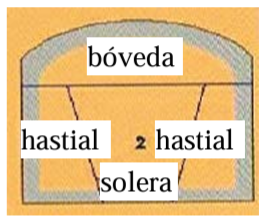
\includegraphics[width=0.5\linewidth]{Imagenes/Tuneles.png}
\end{figure}

% \paragraph{Sostenimiento flexible. Gunitado. Subsidencia. Refuerzos: bulonados y cerchas.}
\paragraph{Movimientos inducidos por túneles: subsidencia.}
La excavación de un túnel altera el estado inicial del terreno generándose movimientos en zonas relativamente próximas a fin de restableces el equilibrio tensional del suelo. En túneles metropolitanos de ferrocarril se han medido asientos de hasta 20 cm.
Fenómenos de subsidencia: son las deformaciones producidas en superficie, originadas por alteraciones en el equilibrio interno del terreno y no por sobrecargas directamente aplicadas en dicha superficie. La subsidencia afecta a edificios con cimentaciones superficiales, pero los movimientos en el interior del terreno (que pueden ser importantes) pueden afectar a cimentaciones profundas. Simplificadamente, son desplazamientos con carácter radial hacia el centro del túnel. Hay diferentes métodos propuestos en la literatura para predecir la subsidencia.

\paragraph{Sostenimiento de la bóveda.}
La bóveda hay que revestirla para proporcionar el apoyo estructural (sostenimiento) necesario, controlar la entrada de agua y ajustar la sección transversal del túnel a las necesidades de operación. Tipos de sostenimiento:
\begin{itemize}
    \item Revestimiento anular de hormigón in situ.
    El gunitado es el proceso de proyección de la gunita por cualquier de los tres sistemas de proyección actualmente existentes (vía seca, vía semi-húmeda y vía húmeda). La gunita se define como ``un mortero u hormigón transportado a través de manguera y proyectado neumáticamente sobre un soporte''. Se suele aplicar en varias capas (de espesor máximo 10 cm aproximadamente para evitar problemas de adherencia; la primera es una capa de sellado. Se suelen armar con un mallazo (Alemania, Austria, Suiza...) o con fibras metálicas (Inglaterra, Suecia, Noruega...)
    
    \item Revestimiento anular hecho con segmentos prefabricados (dovelas).
    Anillo hecho con segmentos prefabricados (dovelas) de fundición o de hormigón masa o armado. \\
    Se colocan inmediatamente detrás de la máquina; una vez colocados se suelen completar con la inyección de mortero en el trasdós. \\
    Tipos de dovelas:
    \begin{itemize}
        \item Dovela de solera: se coloca en la parte inferior del túnel.
        \item Dovelas adyacentes.
        \item Dovelas de contrallave.
        \item Dovelas de clave o llave: última pieza en ser colocada.
    \end{itemize}
    Tipos de anclajes de dovelas:
    \begin{itemize}
        \item Radial: juntas lisas con rebaje, unidas con tornillos de acero.
        \item Circunferencial: juntas entre anillos consecutivos; encaje por presión tuneladora.
    \end{itemize}
    Las juntas entre dovelas reducen la rigidez (presión/deformación racial) del sistema de sostenimiento. (fig. \ref{fig:Dovelas y juntas})

    \begin{figure}[h]
        \centering
        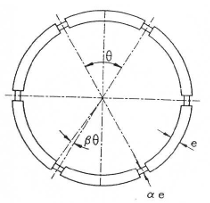
\includegraphics[width=0.5\linewidth]{Imagenes/Dovelas y juntas.png}
        \caption{Dovelas y juntas}
        \label{fig:Dovelas y juntas}
    \end{figure}
   
    \item Revestimientos flexibles a base de bulones (fig. \ref{fig:Bulones}).
    Los bulones son barras de acero (frecuentemente acero corrugado de 25mm) que tienen la misión de unir los estratos alrededor de la sección excavada para formar una bóveda natural. Los bulones quedan anclados por adherencia al mortero o resina de expansión mecánica. El extremo en el exterior del taladro dispone de rosca para tuerca y arandela plana que se ajusta contra la superficie de la roca.

    \begin{figure}[h]
        \centering
        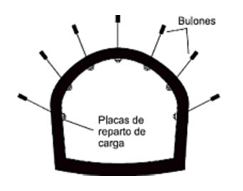
\includegraphics[width=0.5\linewidth]{Imagenes/Revestimiento con bulones.png}
        \caption{Sostenimiento con revestimientos flexibles con bulones.}
        \label{fig:Bulones}
    \end{figure}
    
    \item Revestimiento con cerchas metálicas (fig. \ref{fig:Cerchas Metalicas}.
    Se suelen emplear en macizos rocosos de calidad media. Pueden ser cerchas ligeras, medias o pesadas. Las cerchas deben arriostrase con tresillones. Se emplean en combinación con forros de entibación (chapas continuas o pequeñas tablestacas) o con mallazos cuando se trata de macizos de muy mala calidad. La rigidez de un sistema de cerchas depende mucho de las características del material de acuñado (madera o acero).  
    
    \begin{figure}[h]
        \centering
        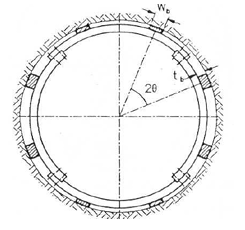
\includegraphics[width=0.5\linewidth]{Imagenes/Sostenimiento con cerchas metalicas.png}
        \caption{Sostenimiento con cerchas metálicas.}
        \label{fig:Cerchas Metalicas}
    \end{figure}
    
\end{itemize}

\subsection{Soluciones convencionales para estructuras e instalaciones industriales.}

\subsubsection{Naves industriales. Puentes grúa.}

\paragraph{Estructuras metálicas porticadas de nudos rígidos.}
Son estructuras que combinan elementos unidimensionales (perfiles metálicos) conectados por nudos rígidos. Es frecuente aumentar la sección de los nudos con cartelas para mejorar su rigidez y capacidad resistente. Para la transmisión de cargas hasta la cimentación se movilizan fundamentalmente esfuerzos de flexión en barras. La rigidez lateral la proporciona el propio pórtico. La rigidez lateral perpendicularmente al plano del pórtico se consigue arriostrando uno o más vanos (con barras diagonales o muros).

\begin{figure}[h]
    \centering
    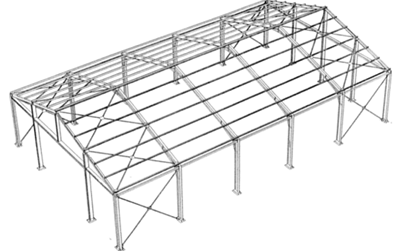
\includegraphics[width=0.75\linewidth]{Imagenes/Est meta de nudos rigidos.png}
    \caption{Estructuras metálicas porticadas de nudos rígidos.}
\end{figure}

\paragraph{Estructuras metálicas trianguladas de nudos articulados: pilares y cerchas.}
Son estructuras que combinan elementos unidimensionales (perfiles metálicos) conectados por nudos articulados. Para transmitir cargas hasta la cimentación se movilizan esfuerzos axiales en las barras. Ventaja: buen aprovechamiento de la sección. Inconveniente: inestabilidad (pandeo) de las barras comprimidas.

\paragraph{Estructuras prefabricadas de hormigón.}

\begin{figure}[H]
    \centering
    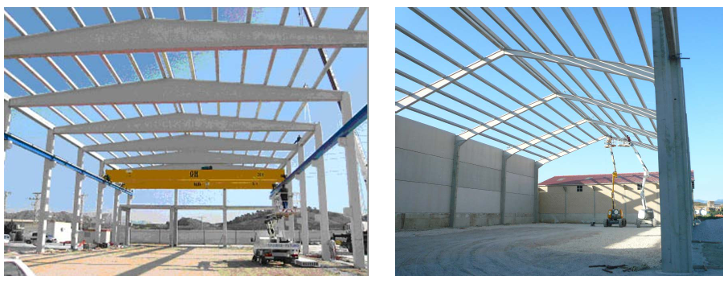
\includegraphics[width=1\linewidth]{Imagenes/Est prefabricadas de hormigon.png}
\end{figure}

\subsubsection{Torres, mástiles y chimeneas. Torres (apoyos) líneas eléctricas.}
Estructura diseñada para soportar las líneas de alta tensión para el transporte y distribución de la energía eléctrica. Soportan los conductores y demás componentes de una línea aérea separándolos del terreno/otras estructuras/etc.

Importancia:
\begin{itemize}
    \item Peligrosida<d de contacto con una línea de alta tensión.
    \item Alta dependencia social del servicio de energía eléctrica.
\end{itemize}

Reglamentos:
\begin{itemize}
    \item 1968: Reglamento de líneas aéreas, aprobado por Decreto 3153/1968, de 28 de Noviembre.
    \item 2008: Reglamento sobre condiciones técnicas y garantías de seguridad en líneas eléctricas de alta tensión, aprobado por Real Decreto 223/2008, de 15 de Febrero.
\end{itemize}

\begin{figure}[h]
    \centering
    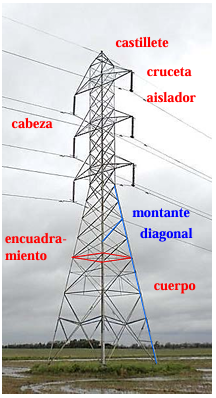
\includegraphics[width=0.5\linewidth]{Imagenes/Torres electricas.png}
    \caption{Partes torre eléctrica.}
\end{figure}

% \paragraph{Tipos.}

\begin{table}[H]
    \centering
    \begin{tabular}{c|c}
         Según su MATERIAL & Según su FUNCIÓN \\
         \hline
         Metálicos & Alineación\\
         Hormigón & Ángulo\\
         Madera & Amarre \\
         Materiales Compuestos & Fin de línea \\
         & Especiales
    \end{tabular}
    \caption{Torres eléctricas. Tipologías.}
\end{table}

\paragraph{Esfuerzos característicos.}
Acciones a considerar:
\begin{itemize}
    \item Cargas permanentes
    \item Fuerza ejercida por el viento
    \item Sobrecargas debidas al hielo
    \item Acción combinada hielo-viento
    \item Desequilibrios de tracciones
    \item Efectos longitudinales por rotura de conductores
    \item Esfuerzos resultantes de ángulo
\end{itemize}

\paragraph{Comprobaciones de seguridad.}
\begin{itemize}
    \item Rotura cables
    \item Vibraciones (uso de amortiguadores y separadores)
    \item Flechas máximas de los conductores y líneas a tierra
    \item Rotura de herrajes
    \item Rotura de aisladores
    \item Resistencia de la torre (Fluencia, resiliencia)
    \item Inestabilidad local y global
\end{itemize}

%\subsubsection{Otras estructuras e instalaciones industriales.}


\section{Estructuras que interaccionan con el suelo: soluciones de cimentación.}

\subsection{Cimentaciones Superficiales.}
\subsubsection{Tipologías.}
Reparte las cargas de las estructura en un plano de apoyo horizontal. Tipos de cimentaciones:
\begin{itemize}
    \item Zapata aislada
    \item Zapata combinada
    \item Zapata corrida
    \item Pozo de cimentación
    \item Emparillado
    \item Losa
\end{itemize}

\begin{figure}[H]
    \centering
    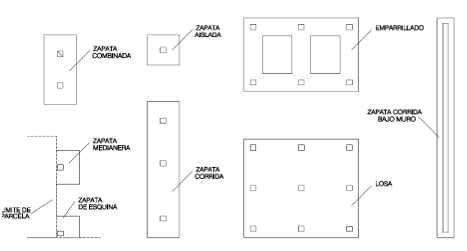
\includegraphics[width=1\linewidth]{Imagenes/Cimentaciones superficiales - Tipos.png}
\end{figure}

\subsubsection{Estados límite de servicio. Bulbo de presiones.}
Asientos del edificio; asientos inducidos en el entorno.
\begin{itemize}
    \item Asieto $s$, definido como el descenso de cualquier punto de la cimentación de un edificio.
    \item Asiento diferencial, $\delta s$, definido como la diferencia de asiento entre dos puuntos cualesquiera de la cimentación.
    \item Distorsión angular, $\beta$, definida como el asiento diferencial entre dos puntos dividido por la distancia que les separa.
    \item Inclinación, $\omega$, definida como el ángulo girado con respecto a la vertical según la línea media que define la posición deformada de la cimentación.
\end{itemize}

Valores límites según CTE.
\begin{table}[H]
    \centering
    \begin{tabular}{p{6cm}|c}
         \hline
         \textbf{Tipo de estructura} & \textbf{Limite} \\
         \hline
         Estructuras isostáticas y muros de contención & 1/300 \\
         Estructuras reticuladas con tabiquería de separación & 1/500 \\
         Estructuras de paneles prefabricados & 1/700 \\
         Muros de carga sin armar con flexión cóncava hacia arriba & 1/1000 \\
         Muros de carga sin armar con flexión cóncava hacia abajo & 1/2000 \\
         \hline
    \end{tabular}
    \caption{Valores límite basados en la distorsión angular.}
\end{table}

\begin{table}[H]
    \centering
    \begin{tabular}{p{6cm}|c}
         \hline
         \textbf{Tipo de estructura} & \textbf{Limite} \\
         \hline
         Muros de carga & 1/2000 \\
         \hline
    \end{tabular}
    \caption{Valores límite basados en la distorsión horizontal}
\end{table}

Cálculo: estudio de presiones en el terreno y proceso de consolidación (se verá en el estudio del suelo como material). Precauciones en el cálculo: Proximidad de las cimentaciones y Bulbo de presiones.

\subsubsection{Estados límite últimos. Presión de hundimiento. Zapatas rígidas y flexibles.}
\begin{itemize}
    \item Hundimiento.
    \item Desplazamiento.
    \item Vuelco.
    \item Estabilidad global.
    \item Capacidad estructural del cimiento.
\end{itemize}

\begin{figure}[H]
    \centering
    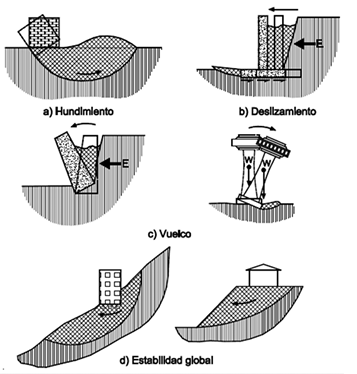
\includegraphics[width=0.75\linewidth]{Imagenes/Cimentaciones superficiales - Estados limite uultimos.png}
\end{figure}

\noindent \underline{Hundimiento. Presión de hundimiento.}

En un cimiento, la aplicación de una carga vertical creciente $V$, da lugar a un asiento creciente. 

Las curvas presión-asiento dependen en general de la forma y tamaño de la zapata, de la naturaleza y resistencia del suelo y de la carga aplicada (tipo, velocidad de aplicación, frecuencia, etc.). 

La carga $V$ para la cual se alcanza el hundimiento es función de la resistencia al corte del terreno, de las dimensiones y forma de la cimentación, de la profundidad a la que está situada, del peso específico del terreno y de las condiciones del agua subálvea.

\begin{figure}[H]
    \centering
    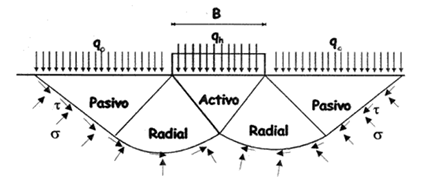
\includegraphics[width=1\linewidth]{Imagenes/Cimentaciones superficiales - estados limite ultimos.png}
\end{figure}

La presión de hundimiento de una cimentación directa vendrá definida por la ecuación (\ref{eq: presion de hundimiento CTE}). Podrá expresarse en presiones totales o efectivas, brutas o netas.
\begin{equation}
    q_h = c_K N_c d_c s_c i_c t_c + q_{0K}N_q d_q s_q i_q t_q + \frac{1}{2}B* \gamma_K N_\gamma d_\gamma s_\gamma i_\gamma t_\gamma
    \label{eq: presion de hundimiento CTE}
\end{equation}
siendo:
\begin{itemize}
    \item $q_h$ la presión vertical de hundimiento o resistencia característica del terreno $R_k$.
    \item $q_{0K}$ la presión vertical característica alrededor del cimiento al nivel de su base.
    \item $c_K$ el valor característico de la cohesión del terreno.
    \item $B*$ el ancho equivalente del cimiento.
    \item $\gamma_K$ el peso específico característico del terreno por debajo de la base del cimiento
    \item $N_c, N_q, N_\gamma$ los factores de capacidad de carga. Son adimensionales y dependen exclusivamente del valor característico del ángulo de rozamiento interno característico del terreno ($\phi_k$). Se denominan respectivamente factor de cohesión, de sobrecarga y de peso específico.
    \item $d_c, d_q, d_\gamma$ los coeficientes correctores de influencia para considerar la resistencia al corte del terreno situado por encima y alrededor de la base del cimiento. Se denominan factores de profundidad.
    \item $s_c, s_q, s_\gamma$ los coeficientes correctores de influencia para considerar la forma en planta del cimiento.
    \item $i_c, i_q, i_\gamma$ los coeficientes correctores de influencia para considerar el efecto de la inclinación de la resultante de las acciones con respecto a la vertical.
    \item $t_c, t_q, t_\gamma$ los coeficientes correctores de influencia para considerar la proximidad del cimiento a un talud.
\end{itemize}

\noindent \underline{Hundimiento. P. caract. en zapatas. Z. rígidas y flexibles.}



\begin{figure}[H]
    \centering
    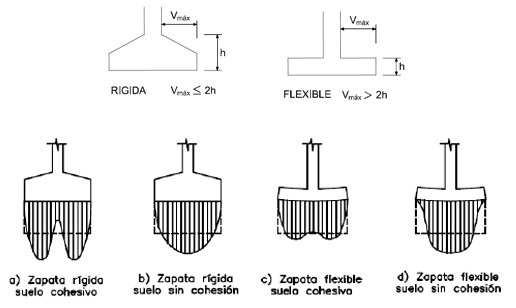
\includegraphics[width=1\linewidth]{Imagenes/Zapatas rigidas y flexibles.png}
\end{figure}

\noindent \underline{Hundimiento. Presión característica en zapatas rígidas.}

\begin{figure}[H]
    \centering
    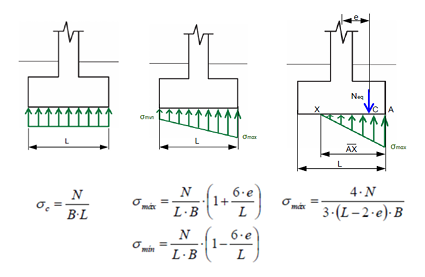
\includegraphics[width=1\linewidth]{Imagenes/Presion caracteristica en zapatas rigidas.png}
\end{figure}

\subsection{Cimentaciones Profundas.}

\subsubsection{Tipologías.}

\subsubsection{Estados límite de servicio.}

\subsubsection{Estados límite últimos. Carga de hundimiento. Efecto grupo.}

\subsection{Estructuras de contención. Muros.}

\subsubsection{Tipologías.}

\subsubsection{Estados límite de servicio.}

\subsubsection{Estados límite últimos.}